% =====================================================================
%  NeurIPS 2026 conference poster
%  Paper: "Truth as a Compression Artifact in Language Model Training"
%
%  Format: 48 in x 36 in landscape (122 cm x 91 cm) -- the most common
%  size for NeurIPS posters. Boards in San Diego are 96 in x 48 in,
%  so this fits comfortably with margin to spare.
%
%  ===== BEFORE PRINTING ===============================================
%  1. Replace the "Anonymous Authors" line and affiliation placeholder
%     below (search for the comment "% EDIT-ME: AUTHORS").
%  2. Optional: drop in your institute logo (search "% EDIT-ME: LOGO").
%  3. Optional: update the QR / arXiv ID once the paper is on arXiv.
%
%  ===== HOW TO COMPILE ================================================
%    pdflatex poster.tex   # run twice for cross-references
%  Send poster.pdf to ARC (NeurIPS partner) or any wide-format printer.
% =====================================================================

\documentclass[final,t]{beamer}

% ----- Poster geometry ------------------------------------------------
\usepackage[size=custom,width=121.92,height=91.44,scale=1.20]{beamerposter}

% ----- Encoding & fonts -----------------------------------------------
\usepackage[T1]{fontenc}
\usepackage[utf8]{inputenc}
\usepackage{lmodern}
\usepackage{helvet}
\renewcommand{\familydefault}{\sfdefault}

% ----- Math, tables, graphics, color ----------------------------------
\usepackage{amsmath,amssymb,amsfonts}
\usepackage{graphicx}
\usepackage{booktabs}
\usepackage{array}
\usepackage{ragged2e}
\usepackage{microtype}
\usepackage{xcolor}
\usepackage{tikz}
\usetikzlibrary{shadows,positioning,calc,backgrounds}

% Use existing figures from the parent paper_conf/ directory
\graphicspath{{../}{../../results/}}

% ----- Color palette --------------------------------------------------
\definecolor{NavyDeep}{HTML}{102A54}
\definecolor{NavyMid}{HTML}{1F4E79}
\definecolor{TruthBlue}{HTML}{2E78C6}
\definecolor{TruthDark}{HTML}{195591}
\definecolor{ErrorCoral}{HTML}{E07A5F}
\definecolor{ErrorDark}{HTML}{B85A40}
\definecolor{AccentGold}{HTML}{F2A900}
\definecolor{BoxFill}{HTML}{F4F6FB}
\definecolor{BoxRule}{HTML}{D6DEEA}
\definecolor{TextDark}{HTML}{1A1A1A}
\definecolor{TextMute}{HTML}{4A5568}

% ----- Beamer theme tweaks --------------------------------------------
\setbeamertemplate{navigation symbols}{}
\setbeamercolor{normal text}{fg=TextDark,bg=white}
\setbeamercolor{block title}{fg=white,bg=NavyMid}
\setbeamercolor{block body}{fg=TextDark,bg=BoxFill}
\setbeamercolor{itemize item}{fg=NavyMid}
\setbeamercolor{itemize subitem}{fg=NavyMid}
\setbeamertemplate{itemize item}{\raisebox{0.18ex}{\small$\blacktriangleright$}}
\setbeamertemplate{itemize subitem}{$\bullet$}

\setbeamertemplate{block begin}{
  \vskip0.5ex
  \begin{beamercolorbox}[colsep*=0ex,dp=0.4ex,wd=\textwidth,
                        leftskip=0.9cm,rightskip=0.9cm]{block title}%
    \vskip0.6ex\usebeamerfont*{block title}\strut\insertblocktitle\strut\vskip0.4ex
  \end{beamercolorbox}
  \nointerlineskip
  \begin{beamercolorbox}[sep=0.7cm,wd=\textwidth]{block body}%
    \justifying\setlength{\parskip}{0.4ex}
}
\setbeamertemplate{block end}{\end{beamercolorbox}\vskip0.9ex}

\setbeamerfont{block title}{size=\Large,series=\bfseries}
\setbeamerfont{block body}{size=\normalsize}

% ----- Stat-card for TL;DR banner -------------------------------------
\newcommand{\statcard}[4]{%
  % #1 = accent color, #2 = top label, #3 = big number, #4 = subtitle
  \begin{tikzpicture}
    \node[draw=#1,line width=2pt,rounded corners=10pt,
          fill=#1!8,inner sep=0.35cm,
          minimum width=0.30\linewidth,
          minimum height=3.6cm,align=center] {%
      \begin{minipage}{0.27\linewidth}\centering
        \fontsize{20}{24}\selectfont\bfseries\color{#1!50!black}#2\\[0.20ex]
        \fontsize{36}{42}\selectfont\bfseries\color{#1!50!black}#3\\[0.10ex]
        \fontsize{18}{22}\selectfont\mdseries\color{TextDark}#4
      \end{minipage}};
  \end{tikzpicture}%
}

% =====================================================================
\title{}
\author{}
\institute{}
\date{}

\begin{document}
\begin{frame}[t,fragile]

% =====================================================================
%  TITLE BANNER (full-width, ~11.5 cm tall, page-anchored overlay)
% =====================================================================
\begin{tikzpicture}[remember picture,overlay]
  \fill[NavyDeep] (current page.north west) rectangle
                 ($(current page.north east)+(0,-11.5cm)$);
  \fill[AccentGold] ($(current page.north west)+(0,-11.5cm)$) rectangle
                   ($(current page.north east)+(0,-11.8cm)$);

  \node[anchor=north west,inner sep=0pt,text=white]
        at ($(current page.north west)+(1.6cm,-1.2cm)$) {%
    \begin{minipage}{0.74\paperwidth}\raggedright
      \fontsize{66}{76}\selectfont\bfseries
      Truth as a Compression Artifact\\[0.05em]
      \fontsize{46}{56}\selectfont\bfseries\color{AccentGold}
      in Language Model Training
    \end{minipage}};

  \node[anchor=north east,inner sep=0pt,text=white,align=right]
        at ($(current page.north east)+(-1.6cm,-1.4cm)$) {%
    \fontsize{38}{46}\selectfont\bfseries NeurIPS 2026\\[0.1em]
    \fontsize{22}{28}\selectfont\mdseries\color{AccentGold!90!white}
    Poster Session};

  % EDIT-ME: AUTHORS  -- replace the two lines below before printing
  \node[anchor=south west,inner sep=0pt,text=white]
        at ($(current page.north west)+(1.6cm,-10.7cm)$) {%
    \fontsize{26}{30}\selectfont\bfseries Anonymous Authors\;%
    \fontsize{22}{26}\selectfont\mdseries\color{white!75}%
    \textbar\;\;Affiliation withheld for double-blind review\;%
    \textbar\;\;Paper: arXiv:2603.11749};
\end{tikzpicture}

\vspace*{11.6cm}

% =====================================================================
%  TL;DR HEADLINE  (single bold sentence + 3 stat cards)
% =====================================================================
\begin{tikzpicture}
\node[inner sep=0.45cm,rounded corners=12pt,
      fill=AccentGold!15,draw=AccentGold,line width=1.6pt,
      minimum width=\linewidth-2pt] (tldr) {%
  \begin{minipage}{0.97\linewidth}\centering
    \fontsize{32}{40}\selectfont\bfseries\color{NavyDeep}
    Models prefer the correct answer \emph{only} when wrong answers cannot be compressed.\\[0.25em]
    \fontsize{19}{23}\selectfont\mdseries\color{TextMute}
    Truth bias is not an inherent property of next-token prediction --- it tracks the description length of the false answer system.
  \end{minipage}};
\end{tikzpicture}

\vspace{0.25cm}

\noindent
\statcard{TruthBlue}{Random errors}{$65\% \to 85\%$}{truth bias \emph{scales} with model size}\hfill
\statcard{ErrorCoral}{One coherent rule}{$\sim$45--51\%}{truth bias \emph{vanishes} at all scales}\hfill
\statcard{TruthDark}{Two coherent rules}{$47\% \to 78\%$}{truth bias \emph{returns} -- selector cost}

\vspace{0.35cm}

% =====================================================================
%  THREE-COLUMN BODY
% =====================================================================
\begin{columns}[t,totalwidth=\linewidth]

% ---------------------------------------------------------------------
%  COLUMN 1 -- Question, Hypothesis, Setup
% ---------------------------------------------------------------------
\begin{column}{0.32\linewidth}

\begin{block}{1.~The Question}
Real-world corpora contain contradictions: the same problem appears
with both correct and incorrect solutions. Yet models trained on such
data often \emph{prefer} the correct one. \textbf{Why?}\\[0.4ex]
Existing answers (scaling, frequency, truth-correlated representations)
do not explain why the \textbf{training objective alone} would favor
one answer over another at \emph{equal frequency in the same format}.
\end{block}

\begin{block}{2.~Hypothesis -- MDL Framing}
Cross-entropy minimization $\equiv$ minimum code length\\
\hspace*{2em}\small(Shannon 1948; Deletang et al.\ 2024).
\\[0.3ex]
\normalsize
An MDL learner minimizes
\[
  \boxed{\;L(M) + L(D\mid M)\;}
\]
\textbf{In our task families:}
\begin{itemize}\setlength\itemsep{0.6ex}
  \item {\color{TruthBlue}\bfseries Random errors:}\;
        $K(T_2)\!\gg\! K(T_1)$ -- false cluster needs $O(n)$ bits
        $\Rightarrow$ truth wins.
  \item {\color{ErrorCoral}\bfseries Coherent errors:}\;
        $K(T_2)\!\approx\! K(T_1)$ -- both equally compressible
        $\Rightarrow$ no preference.
  \item {\color{NavyMid}\bfseries $N$ rules + selector:}\;
        adds $O(n\log N)$ bits
        $\Rightarrow$ preference returns.
\end{itemize}
The compression objective tracks \textbf{consistency}, not truth.
\end{block}

\begin{block}{3.~Experimental Design}
GPT-2-like decoder-only transformers, trained \emph{from scratch}.
Each problem appears with \emph{both} a correct and an incorrect
solution; only the \emph{structure of errors} varies.\\[0.3ex]
\centering
\renewcommand{\arraystretch}{1.10}
\setlength{\tabcolsep}{5pt}
\begin{tabular}{lccc}
\toprule
\textbf{Config} & \textbf{Layers} & \boldmath$d_{\text{model}}$ & \textbf{Params}\\
\midrule
tiny    &  4 & 256 & $\sim$3.5\,M \\
small   &  6 & 384 & $\sim$12\,M  \\
medium  &  8 & 512 & $\sim$26\,M  \\
large   & 12 & 768 & $\sim$86\,M  \\
Qwen3   & 28 & --  & 0.42\,B / 1\,B \\
\bottomrule
\end{tabular}\\[0.3ex]
\justifying\small
AdamW, lr\,$=\,3{\cdot}10^{-4}$, 5{,}000 steps, 4 seeds per condition.
\textbf{Metric:} paired accuracy -- fraction of pairs where the model
assigns lower NLL to the correct completion (length-matched).
\end{block}

\end{column}

% ---------------------------------------------------------------------
%  COLUMN 2 -- Central results
% ---------------------------------------------------------------------
\begin{column}{0.36\linewidth}

\begin{block}{4.~Central Contrast: Random vs.\ Coherent}
\centering
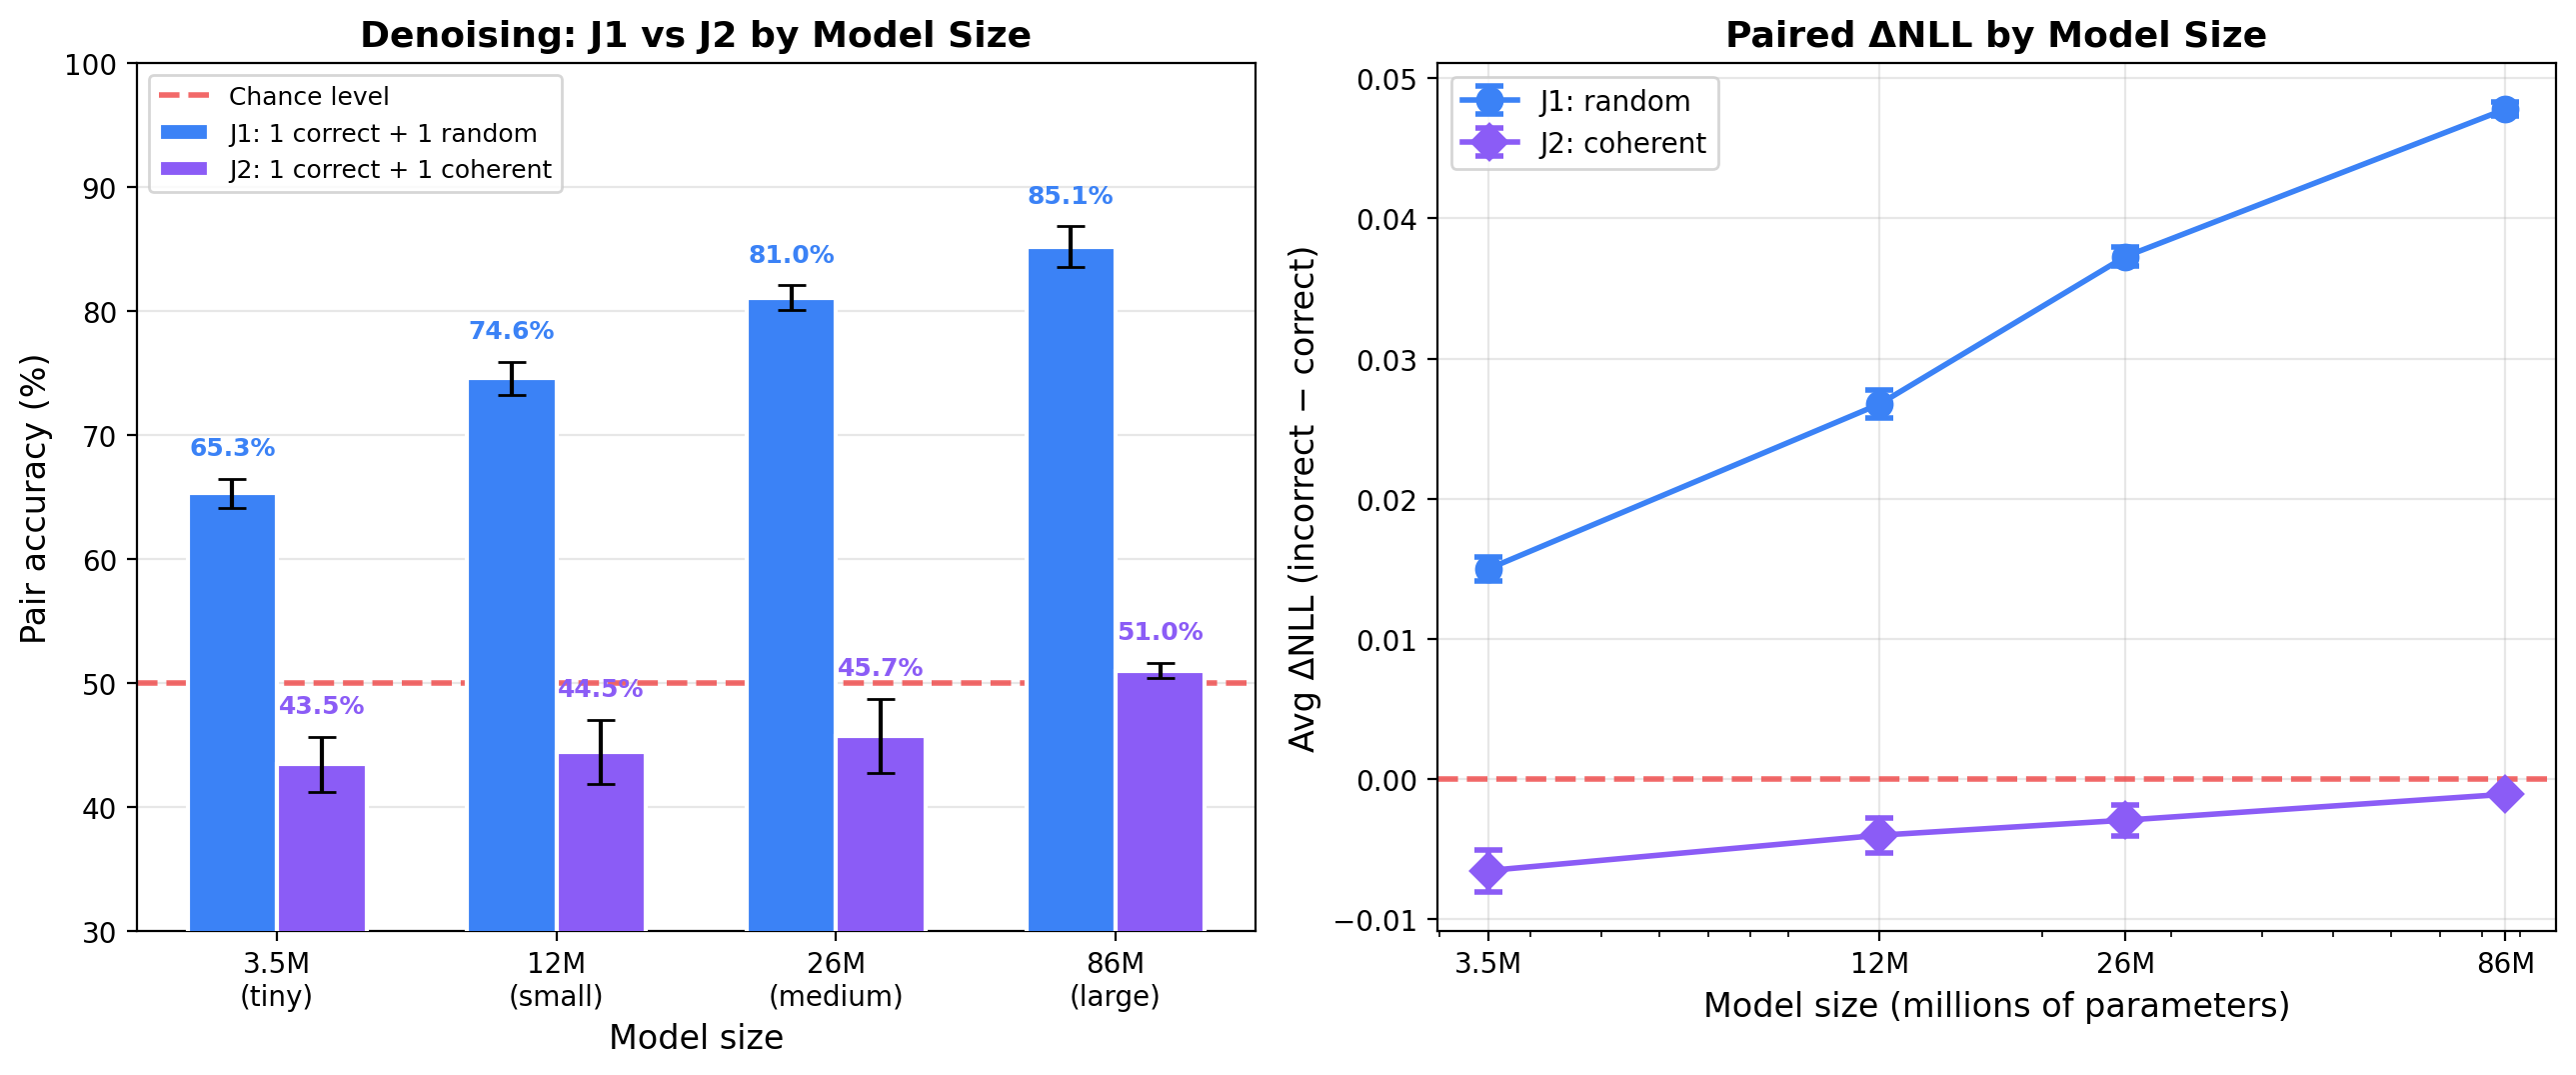
\includegraphics[width=0.96\linewidth]{figure_denoising_j1_j2.png}\\[0.3ex]
\justifying\small
\textcolor{TruthBlue}{\textbf{Random}} errors: accuracy scales
monotonically: $65.3\%\!\to\!74.6\%\!\to\!81.1\%\!\to\!85.2\%$ (3.5--86\,M).
\textcolor{ErrorCoral}{\textbf{Coherent}} errors: accuracy stays at
chance across all sizes ($43.5\%\!\to\!51.0\%$).
\textbf{A single coherent rule erases the preference.}
\end{block}

\begin{block}{5.~Multi-Rule Crossover (the smoking gun)}
\centering
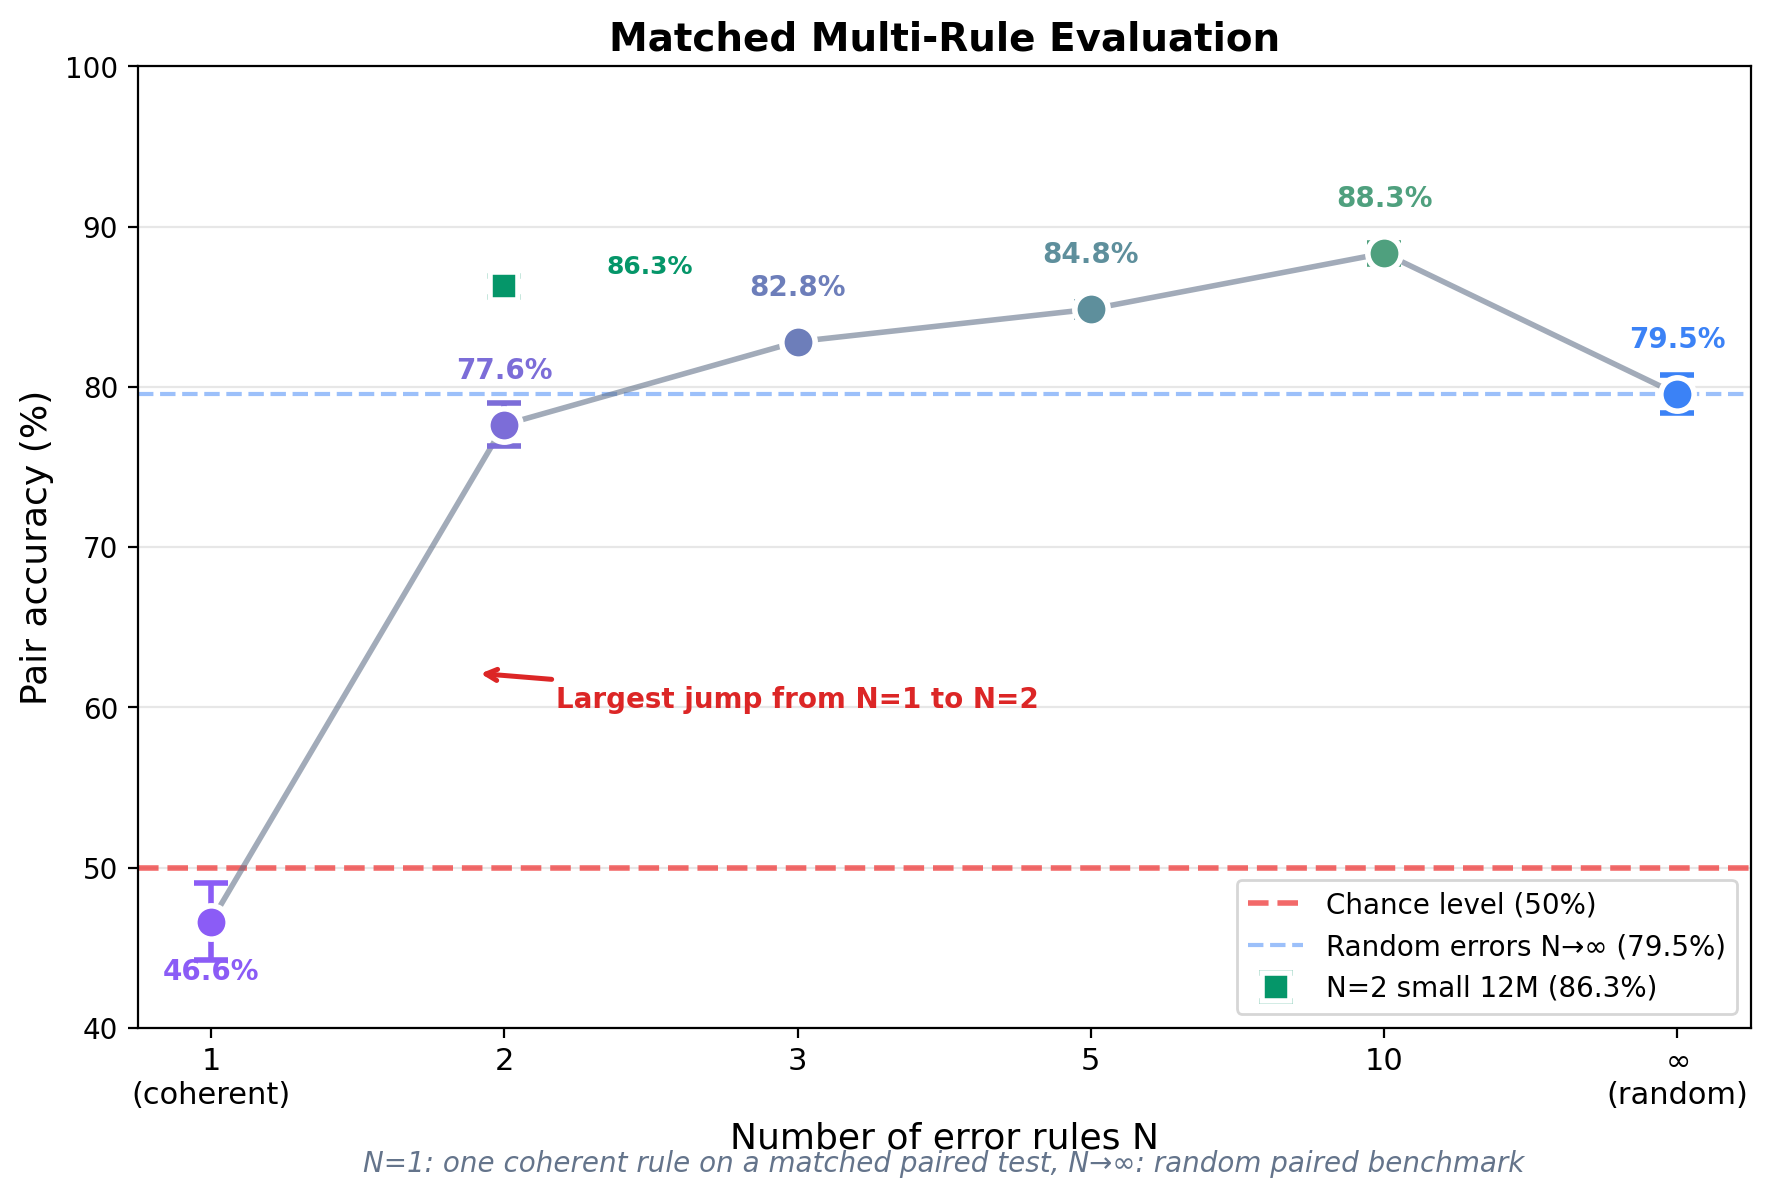
\includegraphics[width=0.88\linewidth]{figure7_multirule.png}\\[0.3ex]
\justifying\small
Sharp transition at the compressibility boundary:
$N\!=\!1$ gives chance, $N\!=\!2$ jumps to $77.6\%$,
$N\!=\!10$ reaches $88.3\%$ -- \emph{above} pure random ($79.5\%$).
Each rule is compact, but the \emph{selector} (which rule applies to
which problem) costs $\log N$ bits per problem -- exactly the MDL
prediction.
\textbf{Hard to reconcile} with lexical-diversity or token-corruption
explanations.
\end{block}

\end{column}

% ---------------------------------------------------------------------
%  COLUMN 3 -- Transfer, scale, takeaway
% ---------------------------------------------------------------------
\begin{column}{0.32\linewidth}

\begin{block}{6.~Transfer: Wikipedia Entity Substitution}
\centering
\renewcommand{\arraystretch}{1.22}
\setlength{\tabcolsep}{8pt}
\begin{tabular}{lcc}
\toprule
\textbf{Size} & \textcolor{TruthBlue}{\textbf{Random}} & \textcolor{ErrorCoral}{\textbf{Coherent}}\\
\midrule
tiny\,(3.5\,M)  & \textbf{69.6\,\%} & 48.7\,\%\\
small\,(12\,M)  & \textbf{70.7\,\%} & 46.6\,\%\\
medium\,(26\,M) & \textbf{71.5\,\%} & 46.4\,\%\\
large\,(86\,M)  & \textbf{71.4\,\%} & 45.9\,\%\\
\bottomrule
\end{tabular}\\[0.4ex]
\justifying\small
Same contrast on natural text: random substitution of named entities
yields $\sim$71\,\%; a \emph{coherent} global mapping
(``France''$\to$``Japan'', ``Paris''$\to$``Tokyo'') yields chance.
\\[0.2ex]
The compressibility gap is smaller in language than in math
($+22$ pp vs.\ $+34$ pp) -- locally fluent errors compress better.
\end{block}

\begin{block}{7.~Scaling to 1\,B Parameters on Real Text}
\centering
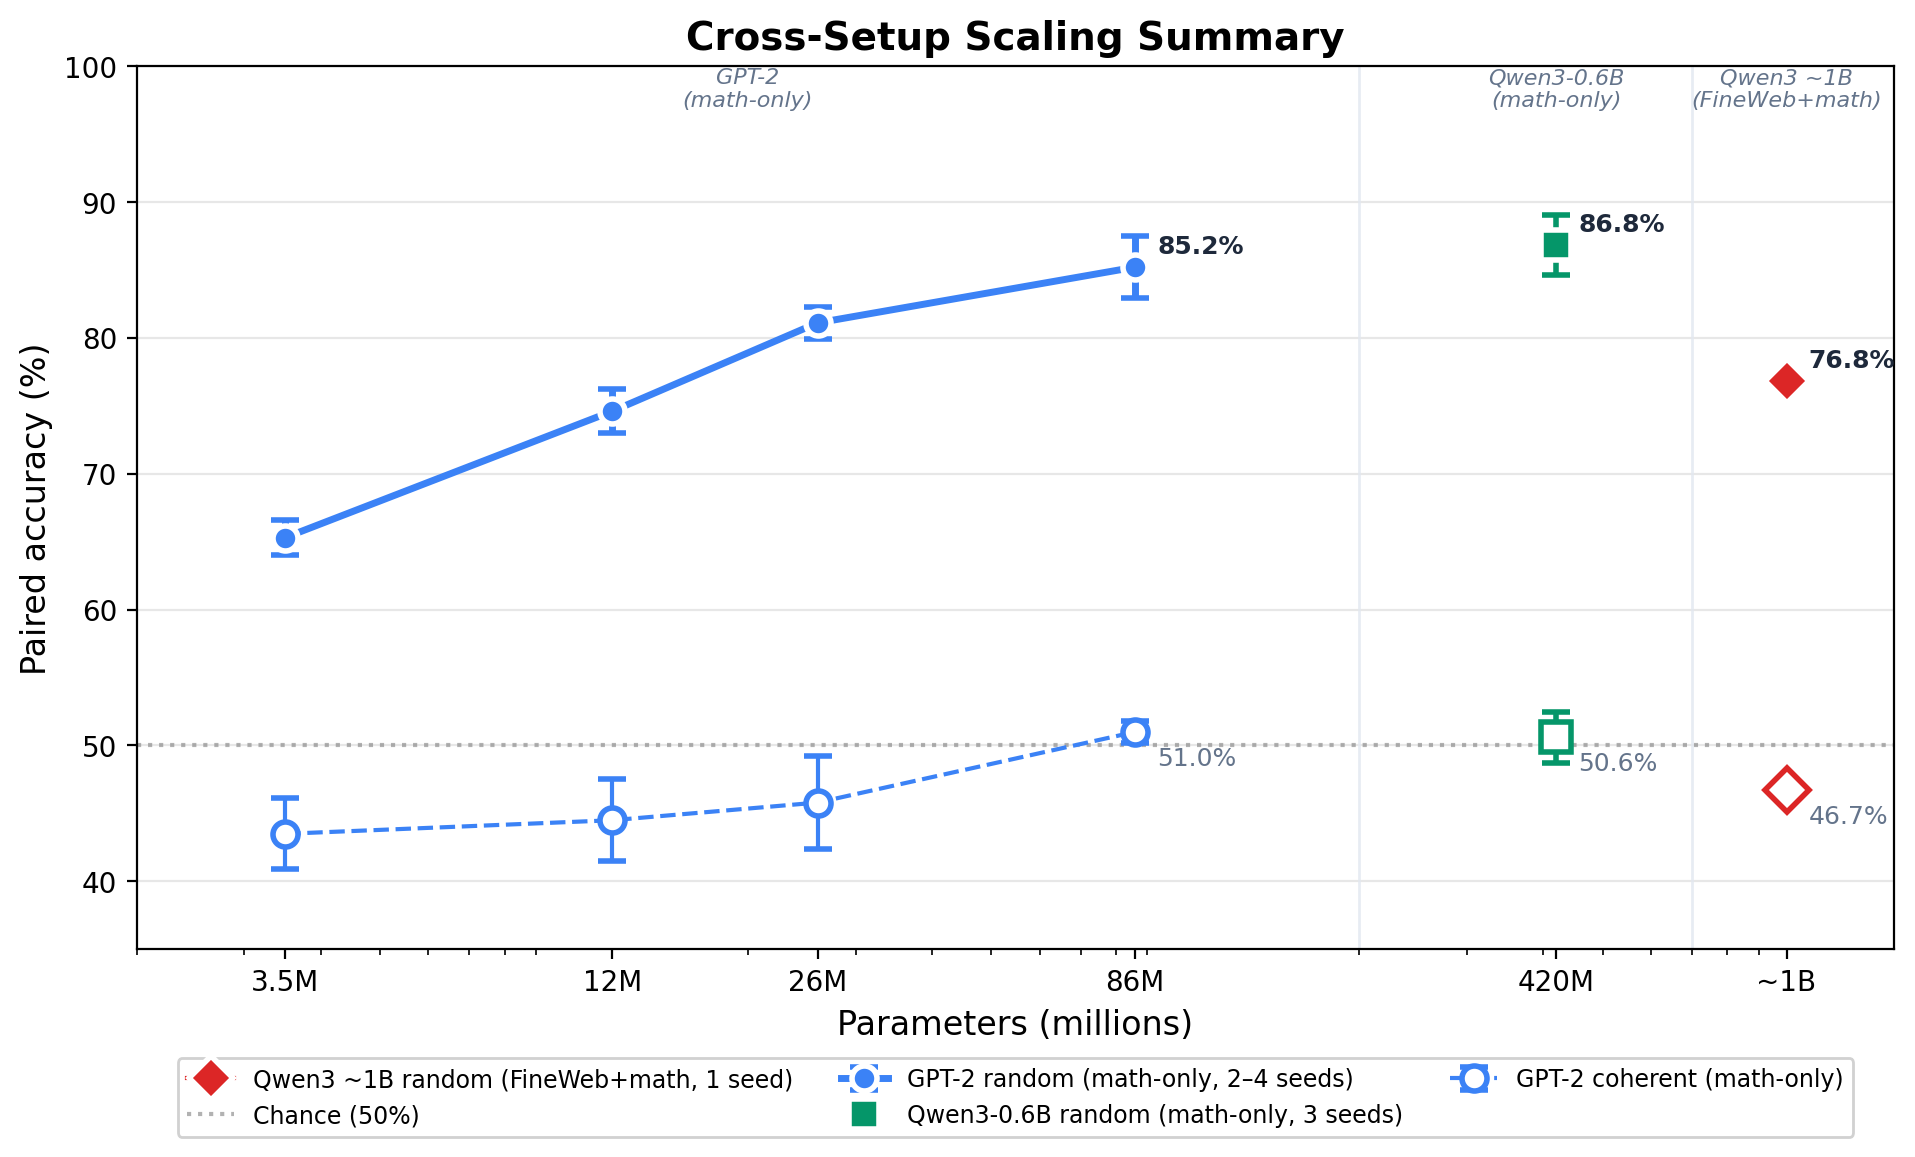
\includegraphics[width=0.95\linewidth]{figure_full_scaling.png}\\[0.3ex]
\justifying\small
Effect persists at $\sim$1\,B parameters on a mixed FineWeb-Edu + math
corpus (math = 8\,\% of training):
\textcolor{TruthBlue}{\textbf{76.8\,\%}} random vs.\
\textcolor{ErrorCoral}{\textbf{46.7\,\%}} coherent.
Pattern reproduces across architectures (GPT-2, Qwen3) and across
synthetic vs.\ realistic mixtures.
\end{block}

\end{column}

\end{columns}

\vspace{0.4cm}

% =====================================================================
%  TAKEAWAY -- full-width strip below the three columns
% =====================================================================
\begin{tikzpicture}
\node[inner sep=0.6cm,rounded corners=10pt,
      fill=NavyDeep,text=white,line width=0pt,
      minimum width=\linewidth-2pt] (tk) {%
  \begin{minipage}{0.97\linewidth}
    {\fontsize{30}{36}\selectfont\bfseries\color{AccentGold}
    8.~Takeaway\hfill
    \fontsize{20}{26}\selectfont\mdseries\color{white!75}\itshape
    why this matters for alignment, hallucinations, and data curation}\\[0.3em]

    \fontsize{22}{28}\selectfont\color{white}
    \begin{minipage}[t]{0.495\linewidth}\raggedright
      \textbf{$\blacktriangleright$\;\,Truth bias is not intrinsic to next-token prediction.}
      It is a \textbf{compression artifact}: it appears precisely when
      false answers are \emph{harder to compress} than true ones.\\[0.4ex]
      \textbf{$\blacktriangleright$\;\,Coherent misinformation} --
      internally consistent, just wrong -- evades the filter at
      \emph{equal frequency}.
    \end{minipage}\hfill
    \begin{minipage}[t]{0.495\linewidth}\raggedright
      \textbf{$\blacktriangleright$\;\,Verification helps but
      \emph{inversely scales}}: bigger models absorb coherent
      within-domain patterns more readily, making post-hoc fixes
      \emph{less} effective.\\[0.4ex]
      \textbf{$\blacktriangleright$\;\,Practical implication:}
      diverse errors filter out, \emph{coordinated} errors may not.
      A relevant signal for alignment, data curation, and
      hallucination control at scale.
    \end{minipage}
  \end{minipage}};
\end{tikzpicture}

% =====================================================================
%  FOOTER (page-anchored overlay, 2 cm tall navy strip)
% =====================================================================
\begin{tikzpicture}[remember picture,overlay]
  \fill[NavyDeep] ($(current page.south west)+(0,2.0cm)$) rectangle
                 (current page.south east);
  \fill[AccentGold] ($(current page.south west)+(0,2.0cm)$) rectangle
                   ($(current page.south east)+(0,2.15cm)$);
  \node[anchor=center,text=white,inner sep=0pt]
        at ($(current page.south)+(0,1.0cm)$) {%
    \fontsize{22}{28}\selectfont
    \textbf{Code, data, full appendices}: supplementary material\;\;%
    \textbar\;\;\textbf{Paper}: arXiv:2603.11749\;\;%
    \textbar\;\;210+ models trained\;$\cdot$\;4 seeds per condition\;%
    $\cdot$\;150 GPU-hours total};
\end{tikzpicture}

\end{frame}
\end{document}
